\subsection{Recommendation: Routing Requests Around the Cache}
\label{sec:recommendation}

The results above establish that only 17.7\% of requests in our trace are faster under blending, and that whether a request wins is governed by its cache hit ratio rather than its size. This raises a practical design question: since the cache path is not universally profitable, can a request be routed \emph{before} it reaches LMCache, so that requests unlikely to benefit go straight to vanilla vLLM? This subsection examines what a routing controller would need to decide, and what the measured data says each decision rule is worth. The question is worth asking precisely because cache reuse costs nothing in output quality, as Section~\ref{sec:ch1_eval} goes on to show, which leaves latency as the only axis on which the routing decision has to be made.

\subsubsection{Is There a Prompt-Length Floor?}
\label{sec:rec_length_floor}

The natural first rule is a prompt-length floor. The intuition is that the cache path carries a startup cost that a short prompt cannot amortize, so below some length the lookup cannot pay for itself even in the best case. Our data supports this intuition, but only under a condition that the rule itself cannot check.

Figure~\ref{fig:crossover} plots median TTFT speedup against prompt length, separately for requests that hit the cache (hit ratio above 70\%) and requests that effectively miss it (hit ratio below 5\%). For the requests that hit, there is a clear crossover. Below roughly 1{,}600 tokens the median speedup is 0.62--0.69$\times$ and no more than a third of requests beat the baseline, because the lookup, onload, and blending machinery costs more than the prefill it avoids. Above that point the median rises to 1.55--2.14$\times$ and the majority of requests beat the baseline, reaching 97--100\% in the two best-sampled buckets. The measured crossover therefore sits near 1{,}600 tokens; we recommend a floor of 2{,}000 tokens, which is deliberately conservative given that the bucket immediately above the crossing contains only four requests.

\begin{figure}[H]
\centering
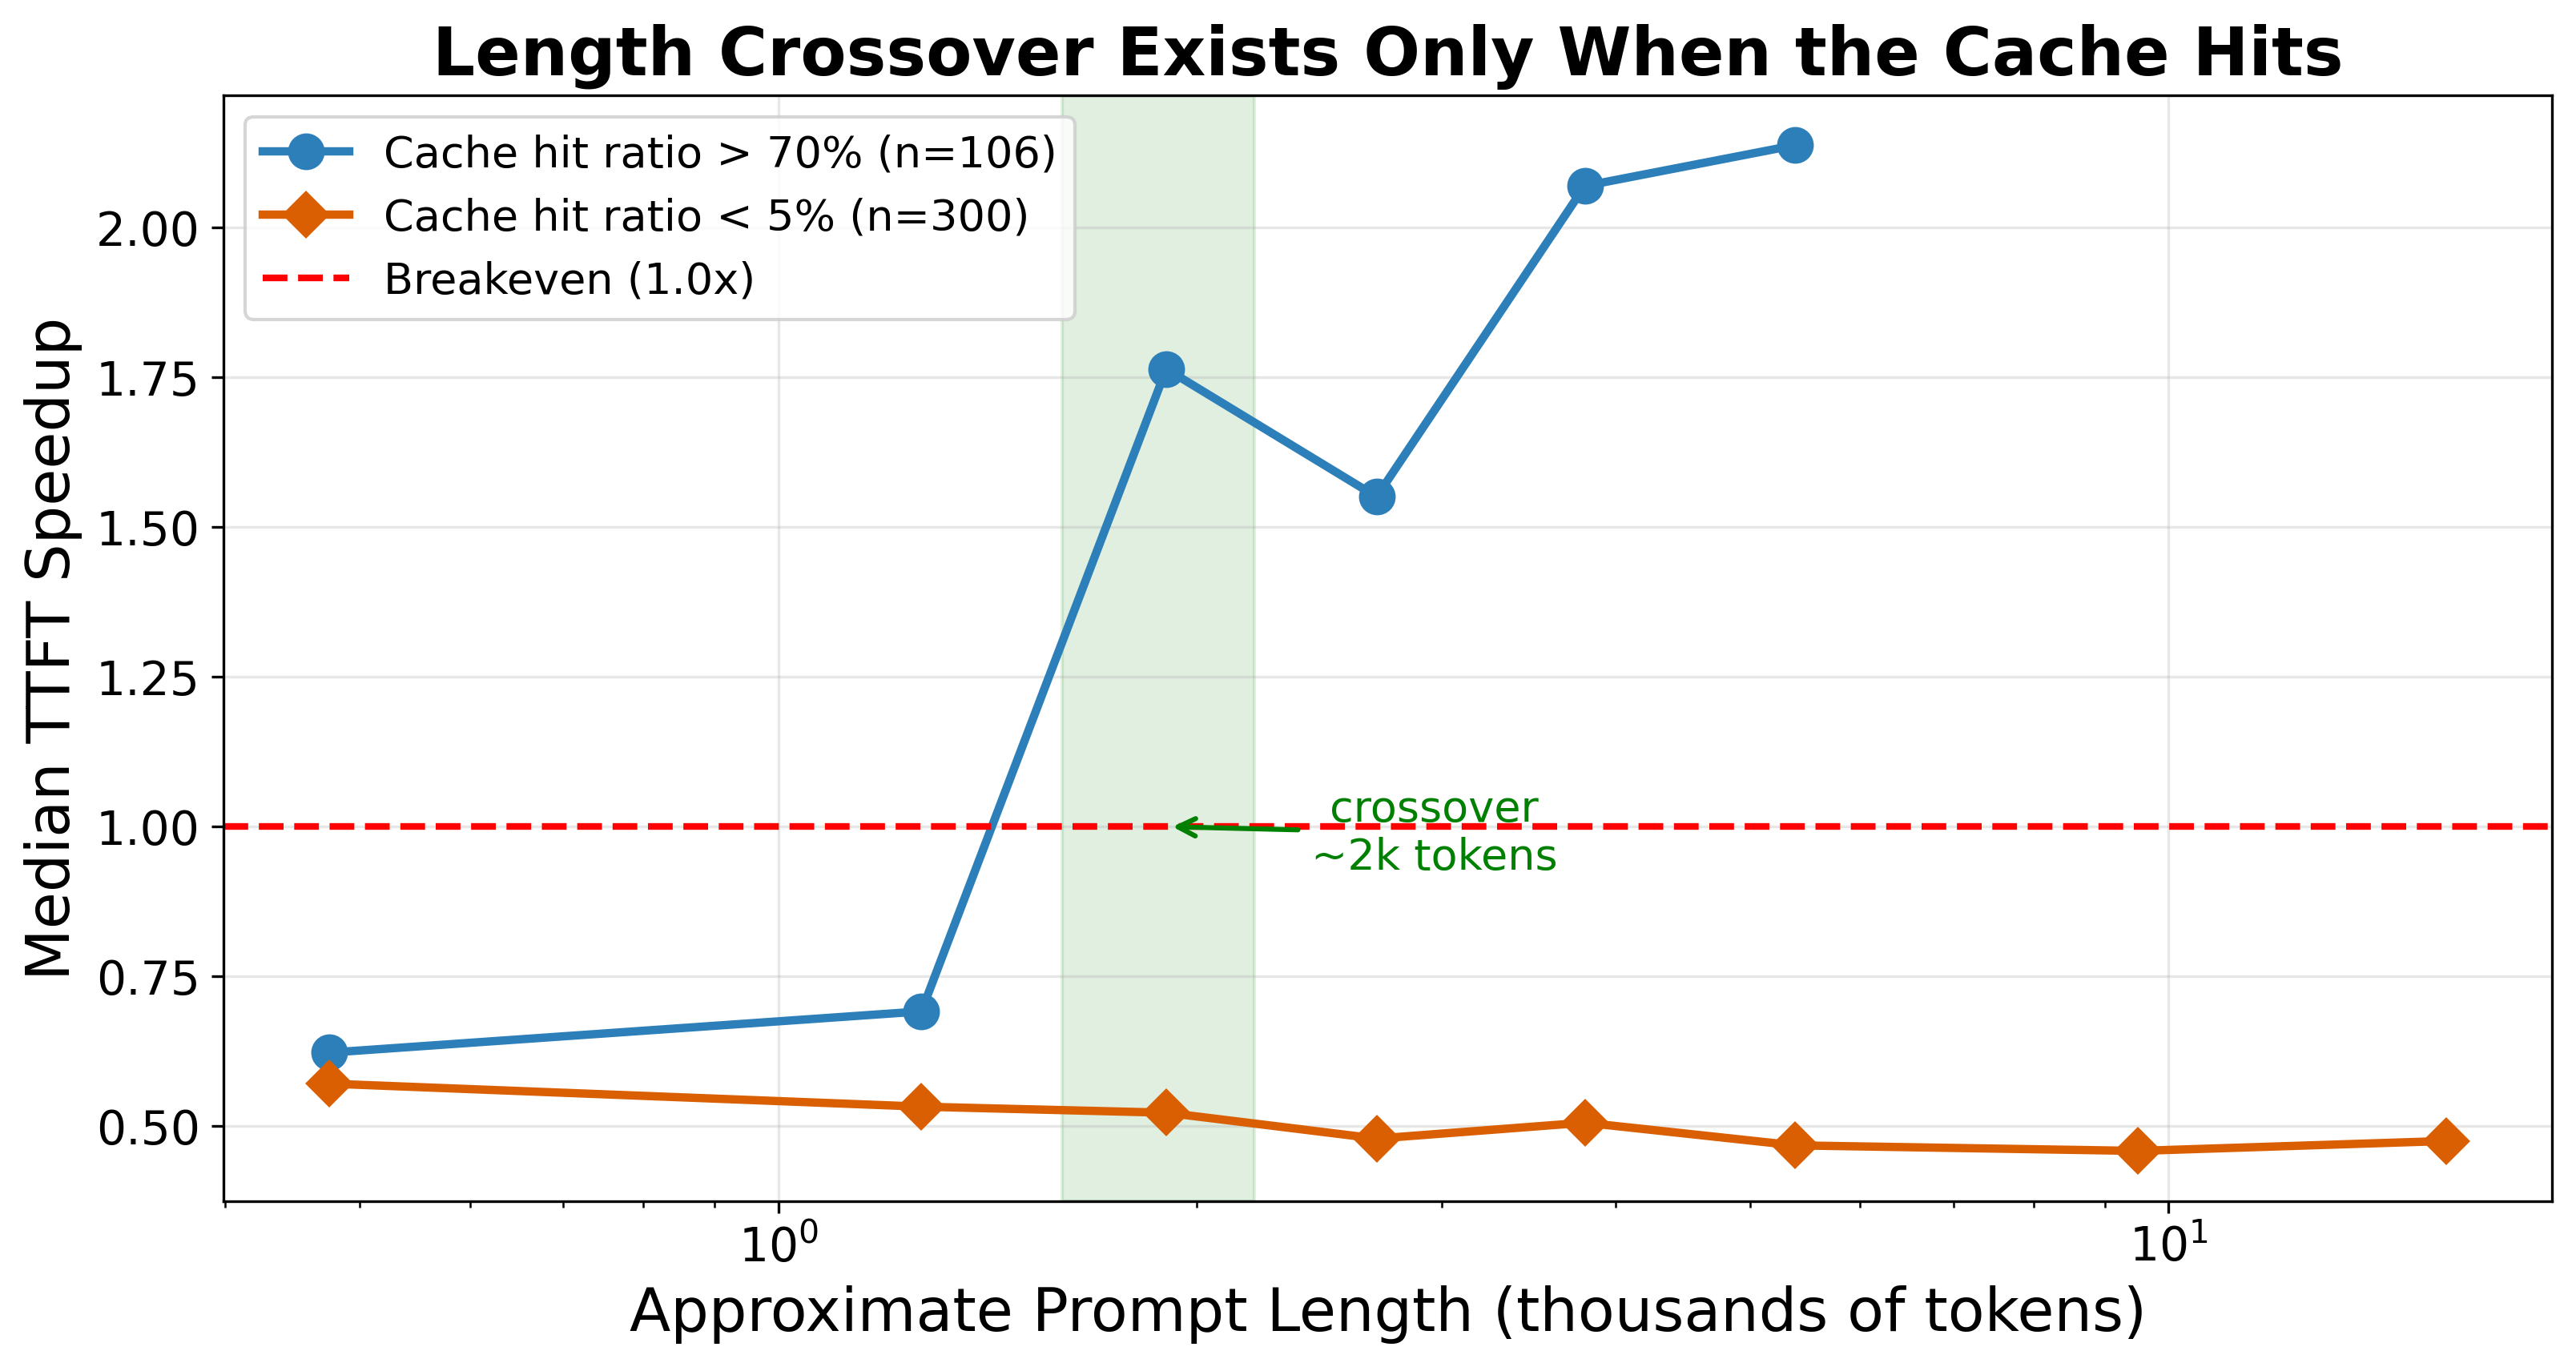
\includegraphics[width=0.9\linewidth]{graphs/thesis_variance_figures/crossover_by_hit_cluster.png}
\vspace{-0.1in}
  \caption{\small Median TTFT speedup vs.\ prompt length, split by cache hit ratio. A length crossover near 2{,}000 tokens exists for requests that hit the cache. For requests that miss, the penalty is flat at ${\sim}0.5\times$ across the entire length range, so no length threshold recovers them. The hit-ratio series ends near 6{,}000 tokens because the trace contains almost no well-cached prompts beyond that length. Prompt length is estimated from baseline TTFT, which is a near-linear proxy (Pearson $r = 0.99$ on the subset with recorded token counts).}
 \label{fig:crossover}
 \vspace{-0.15in}
\end{figure}

For the requests that miss, the picture is entirely different. Their median speedup is 0.46--0.57$\times$ in every length bucket from under 1{,}000 tokens to over 12{,}000 tokens, and essentially none beat the baseline at any length. The penalty for a cache miss is close to scale-invariant: enabling LMCache roughly doubles TTFT whether the prompt is short or long. A length floor therefore cannot help this population, because there is no length at which they stop losing.

\subsubsection{Why the Miss Penalty Does Not Shrink With Length}
\label{sec:rec_miss_penalty}

The scale invariance follows from where the cost is incurred. On a miss, the retrieve path finds nothing and vLLM performs its normal prefill, so the lookup itself is cheap. The expense is on the \emph{store} side. The connector's \texttt{wait\_for\_save} runs the entire GPU-to-CPU offload of the newly computed KV synchronously, and vLLM calls it inside \texttt{execute\_model} before logits are computed and before the sampler runs. The offloaded volume is exactly linear in the number of stored tokens. Every byte of that transfer therefore lands inside TTFT, and it grows in proportion to the prompt, which is why the ratio rather than the absolute penalty is what stays constant.

This is a consequential observation for the controller design, because it means the miss penalty is not an intrinsic property of position-independent reuse. It is a property of storing synchronously on the critical path. Moving the offload to a background stream, so that a request pays only for what it reads and not for what it writes, would remove the penalty for the 80\% of our trace that misses. We did not implement this change, and validating it is the highest-value next step identified by this evaluation.

\subsubsection{What a Length Gate Actually Buys}
\label{sec:rec_gate_effect}

Because the miss population dominates the trace, a length gate alone does not rescue aggregate performance. Figure~\ref{fig:gated_hist} shows the speedup distribution before and after applying the recommended 2{,}000-token floor. The gate bypasses 152 of 536 requests, but the retained distribution is essentially unchanged in shape, and its median speedup moves from 0.509$\times$ to 0.493$\times$. Summed over the trace, routing every request through LMCache costs 772\,s more than vanilla vLLM would have; the best length gate we swept recovers only 28\% of that deficit, and does so by bypassing 77\% of all traffic.

\begin{figure}[H]
\centering
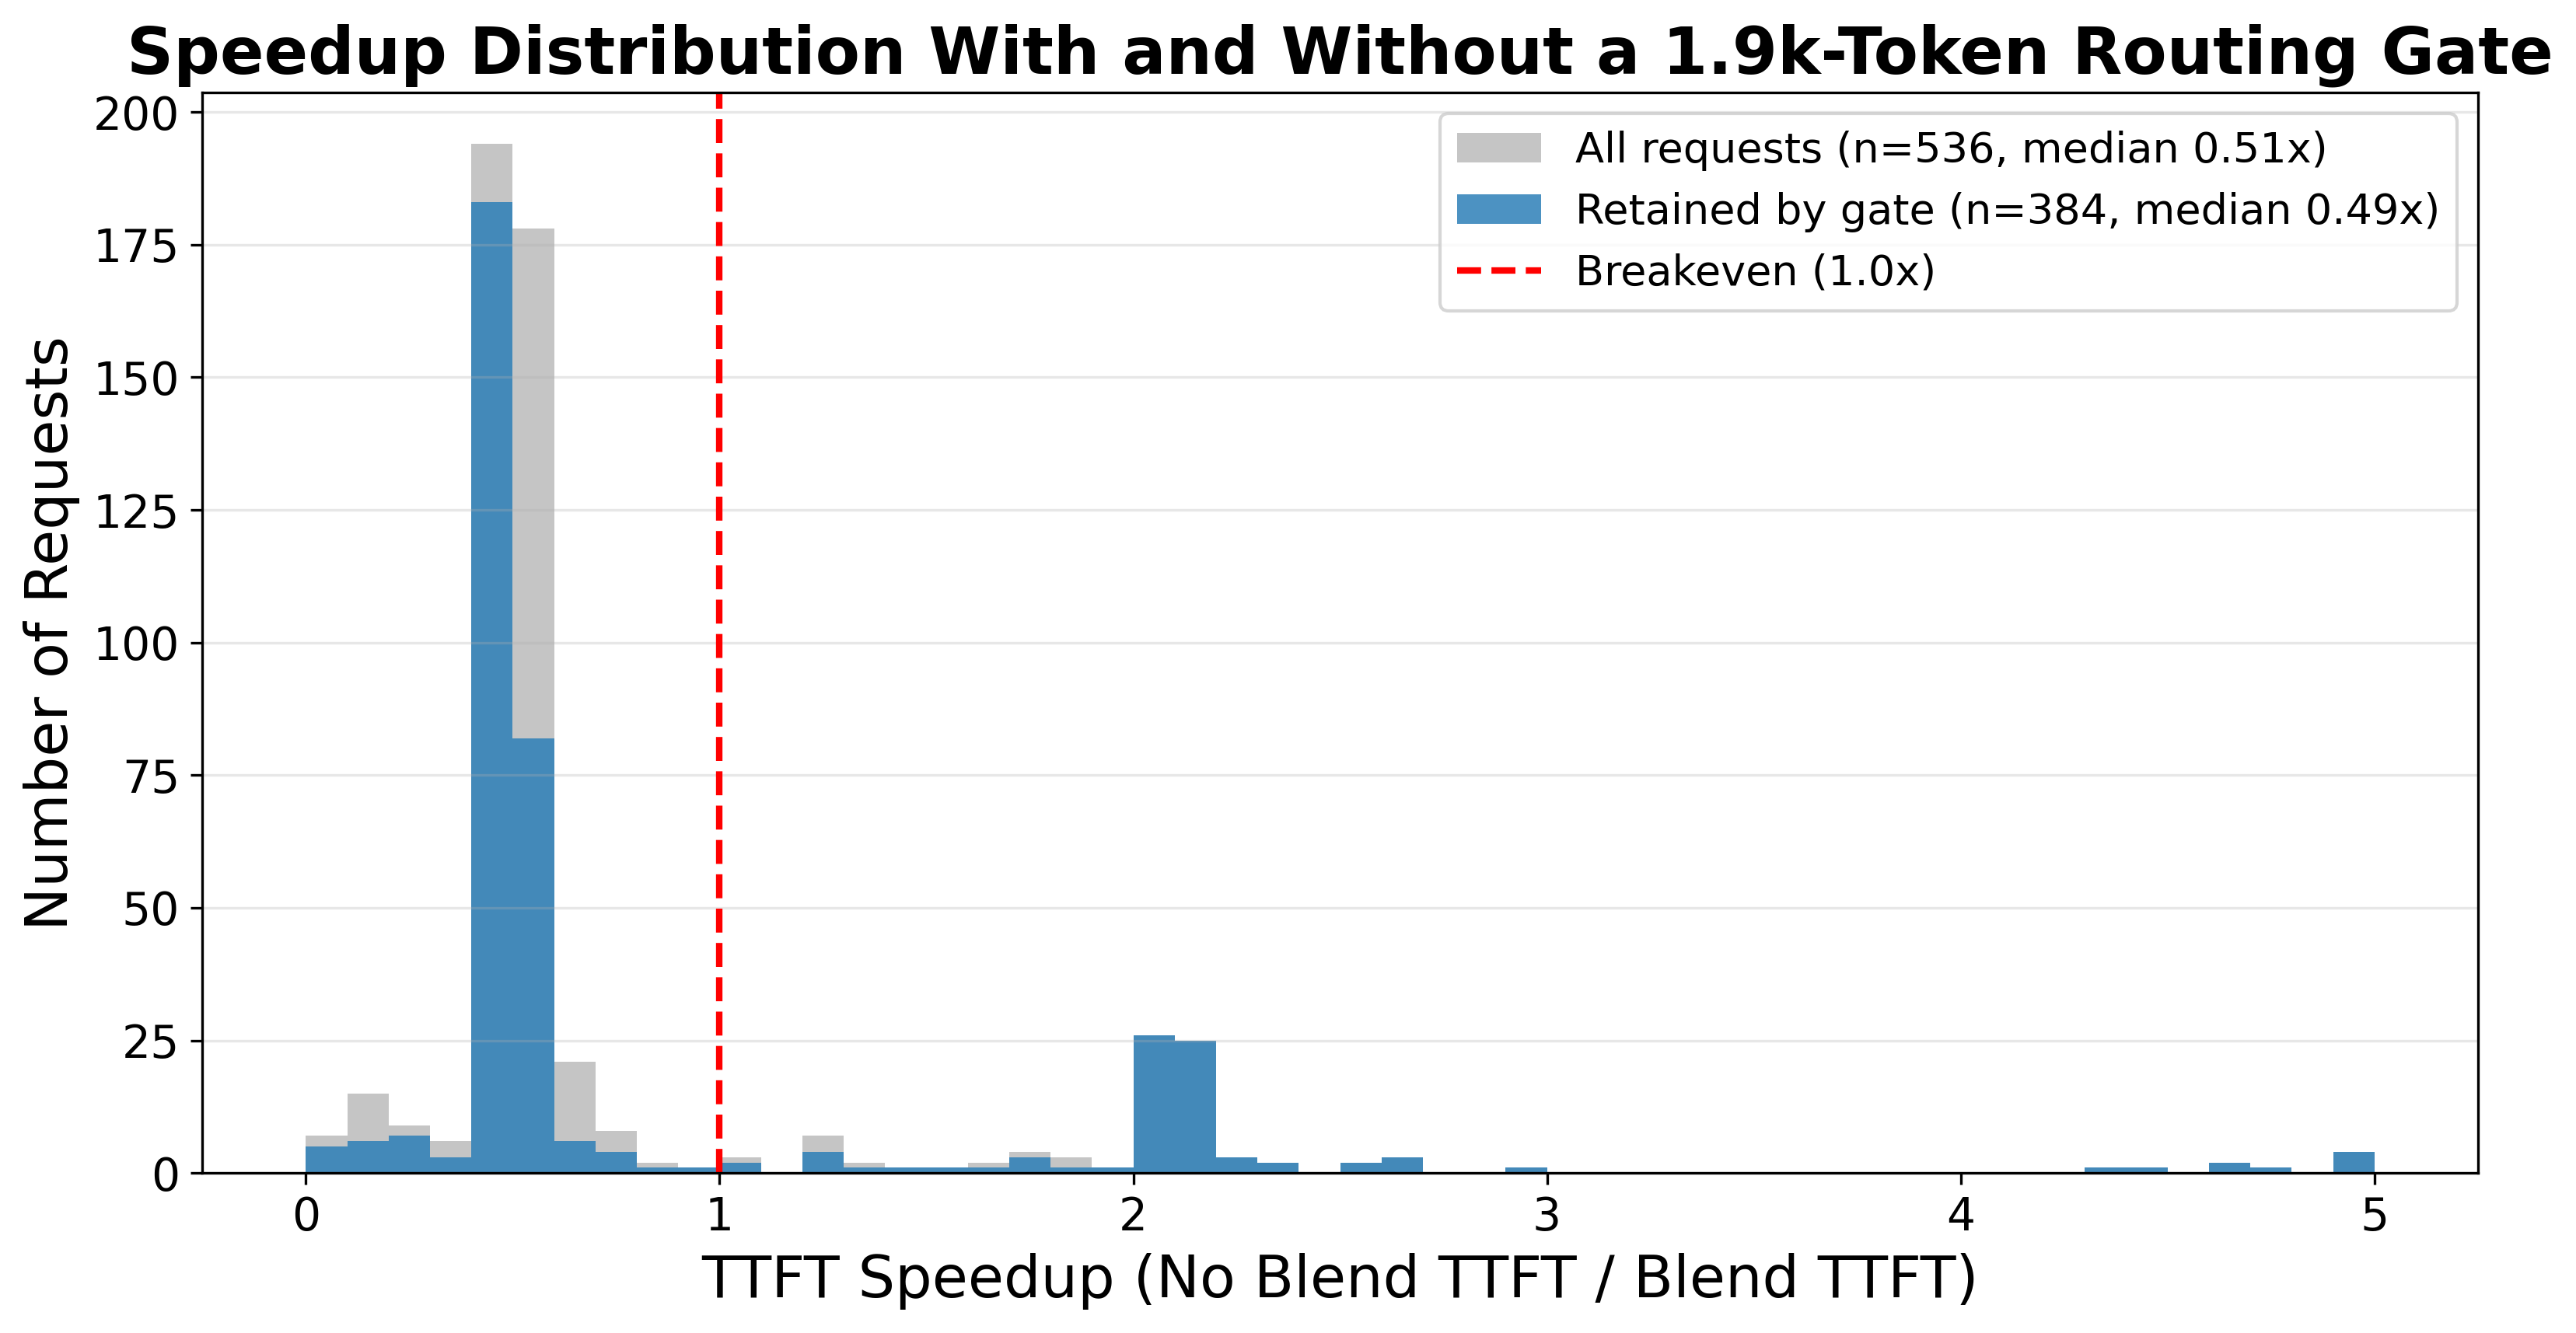
\includegraphics[width=0.9\linewidth]{graphs/thesis_variance_figures/speedup_histogram_length_gated.png}
\vspace{-0.1in}
  \caption{\small Per-request TTFT speedup with and without a 2{,}000-token routing gate. The gate removes requests that cannot win, but the sub-breakeven mode persists because it is populated at all prompt lengths.}
 \label{fig:gated_hist}
 \vspace{-0.15in}
\end{figure}

\subsubsection{Proposed Controller}
\label{sec:rec_controller}

Taken together, these results argue for treating the LMCache layer as optional per request, mediated by a controller in front of the backend that applies two independent rules.

The first is the length floor established above. It is cheap, since prompt length is known before dispatch, and it is safe, since below 2{,}000 tokens the cache path does not win even when it hits. This rule is a strict improvement and can be deployed immediately.

The second rule concerns reuse, and it is the one that determines whether the system is profitable overall. Since the outcome is governed by whether a request will hit, the controller needs an estimate of hit likelihood before committing to the cache path. A cheap approximation is available in the agentic setting: the frontend knows which context objects it assembled into the prompt, so it can report how many of them it has previously sent. That estimate can be attached to the request and used to route. Validating such a predictor requires a trace that samples hit ratio continuously, which ours does not, and we identify this as future work in Section~\ref{sec:conclusion_future}.

Until the store path is made asynchronous, a deployment that cannot predict reuse is better served by enabling LMCache selectively, for workloads known to have high context overlap, rather than by default.

Both rules govern only \emph{whether} a request takes the cache path, never what the model receives, so neither can affect the quality of the generated patch. Section~\ref{sec:ch1_eval} verifies the corresponding property of the cache path itself: that reusing KV state across positions leaves output quality intact.
